%----------------------------------------------------------------------------------------
%	PACKAGES AND OTHER DOCUMENT CONFIGURATIONS
%----------------------------------------------------------------------------------------

\documentclass[twoside]{article}

\usepackage{lipsum} % Package to generate dummy text throughout this template

\usepackage[sc]{mathpazo} % Use the Palatino font
\usepackage[T1]{fontenc} % Use 8-bit encoding that has 256 glyphs
\linespread{1.05} % Line spacing - Palatino needs more space between lines
\usepackage{microtype} % Slightly tweak font spacing for aesthetics

\usepackage[hmarginratio=1:1,top=32mm,columnsep=20pt]{geometry} % Document margins
\usepackage{multicol} % Used for the two-column layout of the document
\usepackage[hang, small,labelfont=bf,up,textfont=it,up]{caption} % Custom captions under/above floats in tables or figures
\usepackage{booktabs} % Horizontal rules in tables
\usepackage{float} % Required for tables and figures in the multi-column environment - they need to be placed in specific locations with the [H] (e.g. \begin{table}[H])
\usepackage{hyperref} % For hyperlinks in the PDF

\usepackage{lettrine} % The lettrine is the first enlarged letter at the beginning of the text
\usepackage{paralist} % Used for the compactitem environment which makes bullet points with less space between them

\usepackage{abstract} % Allows abstract customization
\renewcommand{\abstractnamefont}{\normalfont\bfseries} % Set the "Abstract" text to bold
\renewcommand{\abstracttextfont}{\normalfont\small\itshape} % Set the abstract itself to small italic text

\usepackage{titlesec} % Allows customization of titles
\renewcommand\thesection{\Roman{section}} % Roman numerals for the sections
\renewcommand\thesubsection{\Roman{subsection}} % Roman numerals for subsections
\titleformat{\section}[block]{\large\scshape\centering}{\thesection.}{1em}{} % Change the look of the section titles
\titleformat{\subsection}[block]{\large}{\thesubsection.}{1em}{} % Change the look of the section titles

\usepackage{fancyhdr} % Headers and footers
\pagestyle{fancy} % All pages have headers and footers
\fancyhead{} % Blank out the default header
\fancyfoot{} % Blank out the default footer
\fancyhead[C]{ESE650 Learning in Robotics $\bullet$ February 2014 $\bullet$ Project 2} % Custom header text
\fancyfoot[RO,LE]{\thepage} % Custom footer text

\usepackage[pdftex]{graphicx}
\usepackage{subfigure}
\usepackage{amsmath,amssymb,amsopn,amstext,amsfonts}
\usepackage{url}
\usepackage[usenames,dvipsnames]{color}
\usepackage{siunitx}
\usepackage{amsmath}
\usepackage{amsfonts}
\usepackage{amssymb}

\graphicspath{{fig/}}
\newcommand{\W}{\mathcal{W}}
\newcommand{\X}{\mathcal{X}}
\newcommand{\Y}{\mathcal{Y}}
\newcommand{\Z}{\mathcal{Z}}
\newcommand{\red}[1]{\textcolor{red}{#1}}
\newcommand{\brown}[1]{\textcolor{brown}{#1}}
%----------------------------------------------------------------------------------------
%	TITLE SECTION
%----------------------------------------------------------------------------------------

\title{\vspace{-15mm}\fontsize{24pt}{10pt}\selectfont\textbf{Orientation Tracking}} % Article title

\author{
\large
\textsc{Chao Qu}\thanks{A thank you or further information}\\[2mm] % Your name
\normalsize University of Pennsylvania \\ % Your institution
\normalsize \href{mailto:quchao@seas.upenn.edu}{quchao@seas.upenn.edu} % Your email address
\vspace{-5mm}
}
\date{}

%----------------------------------------------------------------------------------------

\begin{document}


\maketitle % Insert title

\thispagestyle{fancy} % All pages have headers and footers

%----------------------------------------------------------------------------------------
%	ABSTRACT
%----------------------------------------------------------------------------------------

%\begin{abstract}
%
%\noindent Hey, I'm just an abstract. % Dummy abstract text
%
%\end{abstract}

%----------------------------------------------------------------------------------------
%	ARTICLE CONTENTS
%----------------------------------------------------------------------------------------

%----------------------------------------------------------------------------------------
%	INTRODUCTION
%----------------------------------------------------------------------------------------

\begin{multicols}{2} % Two-column layout throughout the main article text

\section{Introduction}
\lettrine[nindent=0em,lines=2]{O}rientation Tgracking

%----------------------------------------------------------------------------------------
%	PRE-PROCESSING
%----------------------------------------------------------------------------------------

\section{Pre-processing}
The raw IMU data we get is 10-bit ADC values, which technically ranges from 0 to 1023. Since it's difficult to use those values directly in our filter, we have to convert them so that they have real-world physical units and meanings. Our goal here is to convert the readings from the micro-controller to acceleration with a unit of \si{m/s^2} and angular velocity with a unit of \si{\radian/s}.
The equations used for converting raw values to real values are shown in Eq.\ref{eq:convert_acc} and Eq.\ref{eq:convert_omg}.
\begin{align}
\label{eq:convert_acc}
\vec{a} &= (\vec{a}_{raw} - \vec{a}_{bias}) \cdot s_{a}\\
\vec{\omega} &= (\vec{\omega}_{raw} - \vec{\omega}_{bias}) \cdot s_{\omega}
\label{eq:convert_omg}
\end{align}
where 
\begin{equation}
\vec{a}_{bias} = \begin{bmatrix}511.5 & 511.5 & 511.5\end{bmatrix}
\end{equation}
and $\vec{\omega}_{bias}$ is determined empirically by averaging the first 100 readings of one of the IMU data
\begin{equation}
\vec{\omega}_{bias} = \begin{bmatrix}373.63 & 375.20 & 369.66\end{bmatrix}
\end{equation}
$s_{a}$ and $s_{\omega}$ are the scale factors and their values are $0.0106$ and $0.0171$.

We then look at the rotations in details.
\begin{figure}[H]
\centering
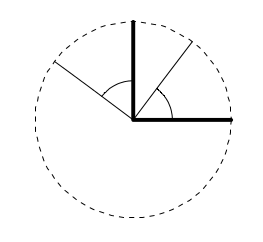
\includegraphics[width=0.5\columnwidth]{fig/rot.png} 
\caption{A simple rotation along z-axis, with angle $\psi$}
\label{fig:rotz}
\end{figure}
Assume at some time $t_0$, the IMU is perfectly aligned with the world frame. In the next time step $t_0+\Delta t$, there's a very small rotation along the z-axis, and the gyro thus measures an angular velocity $\omega_z$, and thus an angle $\Psi = \omega_z \cdot \Delta t$. This is shown in Fig.\ref{fig:rotz}. The rotation matrix of the rotation is denoted by $R_z(\psi)$ and it physically rotates the world SRT into the body SRT. Thus we call the rotation matrix \textit{World-to-Body} and written in $^BR_W$. If there's rotation in all 3 axes, then we use a sequence of euler angles to indicate angular movement along each axis and this can be written as
\begin{equation}
^BR_W = R_x(\phi)R_y(\theta)R_z(\psi)
\end{equation}
where each of them is
\begin{equation}
R_x(\phi) = \left(\begin{array}{ccc} 1 & 0 & 0\\ 0 & \cos\!\left(\phi{}\right) & \sin\!\left(\phi{}\right)\\ 0 & - \sin\!\left(\phi{}\right) & \cos\!\left(\phi{}\right) \end{array}\right)
\end{equation}
\begin{equation}
R_y(\theta) = \left(\begin{array}{ccc} \cos\!\left(\theta{}\right) & 0 & - \sin\!\left(\theta{}\right)\\ 0 & 1 & 0\\ \sin\!\left(\theta{}\right) & 0 & \cos\!\left(\theta{}\right) \end{array}\right)
\end{equation}
\begin{equation}
R_z(\psi) = \left(\begin{array}{ccc} \cos\!\left(\psi{}\right) & \sin\!\left(\psi{}\right) & 0\\ - \sin\!\left(\psi{}\right) & \cos\!\left(\psi{}\right) & 0\\ 0 & 0 & 1 \end{array}\right)
\end{equation}
and we also notice that if the world coordinates and body coordinates of the gravity vector can be related by this rotation matrix
\begin{equation}
\begin{Bmatrix}0 \\ 0 \\ g\end{Bmatrix} = 
^WR_B \begin{Bmatrix}a_x \\ a_y \\ a_z\end{Bmatrix}
\end{equation}
where $a_x$, $a_y$ and $a_z$ are measurements by the accelerometer.
%----------------------------------------------------------------------------------------
%	METHODS
%----------------------------------------------------------------------------------------

\section{Methods}
For the main unscented kalman filter algorithm, I basically followed the steps outlined in Kraft's paper \cite{Kraft03}. For calculating quaternion mean, I used the method proposed by Cheon \cite{Cheon07} instead of gradient descent. Another difference is that Kraft uses only $2n$ Sigma points with uniform weights, while Cheon uses $2n+1$ Sigma points with weights determined by parameters such as $\alpha$, $\beta$ and $\kappa$. Here I will describe the algorithm in detail. The following content is either from Kraft or from Cheon. It focuses more on the steps and implementations than the underlying theorems and principles, which serves the purpose for my personal review later.

\subsection{Process Model}
Process model in kalman filter takes the from
\begin{equation}
x_{k+1} = A(x_k, w_k)    
\end{equation}
where $x$ is the state vector and $w$ is the process noise with $0$ mean and covariance $Q$. The first 3 components of $w_k$ affect the orientation and the last three components of $w_k$ affects angular velocity.
\begin{equation}
w_k = \begin{pmatrix}\vec{w}_q \\ \vec{w}_\omega \end{pmatrix}
\end{equation}
The final process model is 
\begin{equation}
x_{k+1} = A(x_k, w_k) = \begin{pmatrix} q_k q_w q_{\Delta}\\ \vec{\omega}_k + \vec{w}_\omega \end{pmatrix}
\end{equation}
where $q_k$ is the quaternion of the previous time step and $q_w$ is the quaternion representing process noise
\begin{align}
q_w &= \begin{bmatrix}
\cos\left(\alpha_w/2\right) & \vec{e}_w \sin \left(\alpha_w/2 \right)\end{bmatrix}\\
\alpha_w &= \|w_q\|, \quad \vec{e}_w = \frac{w_q}{\|w_q\|}
\end{align}
and $q_\Delta$ is the quaternion representing the rotation during the interval of sensor update
\begin{align}
q_\Delta &= \begin{bmatrix}
\cos\left(\alpha_\Delta/2\right) & \vec{e}_\Delta \sin \left(\alpha_\Delta/2\right)\end{bmatrix}\\
\alpha_\Delta &= \|\vec{\omega}_k\|\cdot \Delta t, \quad \vec{e}_\Delta = \frac{\vec{\omega}_k}{\|\vec{\omega}_k|}
\end{align}

\subsection{Measurement Model}
Measurement model in kalman filter takes the from
\begin{equation}
z_k = H(x_k, v_k)
\end{equation}
Since we have gyro and accelerometer, we have two different type of measurement. The two measurement models are
\begin{align}
H_1: \quad \vec{z}_{rot} &= \vec{\omega}_k + \vec{v}_{rot} \\
H_2: \quad \vec{z}_{acc} &= \vec{g'} + \vec{v}_{acc} 
\end{align}
where
\begin{align}
&g' = q_k g q_k^{-1} \\
&g  = (0,\;[g_x,g_y,g_z])
\end{align}
and $[g_x,g_y,g_z]$ is the acceleration readings from the IMU.

\subsection{Initialization}
At the initialization step, we first initialize the state vector to be
\begin{equation}
x_0 = \begin{pmatrix}q_0 \\ \omega_0\end{pmatrix}
=\begin{bmatrix}
1 & 0 & 0 & 0 & 0 & 0 & 0
\end{bmatrix}^\top
\end{equation}
because we roughly know that at the beginning the platform is stationary on the ground. Then we generates the weights $W^{(m)}$ and $W^{(c)}$ using the following parameters
\begin{equation}
\alpha = 0.5, \quad \beta = 2, \quad \kappa = 0
\end{equation}
Details for calculating the weights can be found in \cite{Julier97}. We then initialize the state covariance $P$, process covariance $Q$ and measurement covariance $R$, all of them are $6\times6$ diagonal matrices.

\subsection{Prediction}
At the prediction step, given the state vector $x_k$, state covariance $P_k$ and process covariance $Q_k$, we calculate a set of $(2n+1)$ sigma points $\X_i$ using the following equations
\begin{equation}
\X_i = \begin{pmatrix}q_k & q_k q_\W \\ \vec{\omega}_k & \vec{\omega}_k + \vec{\omega}_\W\end{pmatrix}
\end{equation}
in which
\begin{align}
\W_i          &= \mbox{columns}(\pm \gamma \sqrt{P_k + Q_k}) \\
\gamma        &= \sqrt{n+\lambda}, \quad n = 6 \\
\lambda       &= \alpha^2(n+\kappa) - n \\
\W_{i,q}      &= \mbox{first 3 rows}(\W_i) \\
\W_{i,\omega} &= \mbox{last 3 rows}(\W_i) = \vec{\omega}_\W
\end{align}
then
\begin{align}
q_\W &= \begin{bmatrix}\cos(\alpha_\W/2) & \vec{e}_\W \sin(\alpha_\W/2)\end{bmatrix} \\
\alpha_\W &= \|\W_{i,q}\|, \quad \vec{e}_\W = \frac{\W_{i,q}}{\|\W_{i,q}\|}
\end{align}
We then transform the sigma points ahead of time through the process model
\begin{equation}
\Y_i = A(\X_i,0)
\end{equation}
using the process model we described in previous section.
The set $\{\Y_i\}$ samples the probability distribution of the \textit{a priori} estimate. And the mean and covariance of this distribution are
\begin{align}
\hat{x}^-_k &= \mbox{mean}(\{\Y_i\}) \\
P^-_k &= \mbox{cov}(\{\Y_i\})
\end{align}
Calculating the mean of quaternions is a little bit tricky in this case. Instead of using a gradient descent method, we use a barycentric mean with renormalization which is proposed in \cite{Cheon07}. The equation for calculating quaternion mean is
\begin{equation}
\hat{q}^-_k = \frac{\sum^{2n}_{i=0}W_i \Y^q_i}{\|\sum^{2n}_{i=0}W_i \Y^q_i\|}
\end{equation}
This ensures that the result quaternion mean also lies on the unit quaternion sphere.
We then need to calculate covariance $P^-_k$, this is done by 
\begin{equation}
P^-_k = \sum^{2n}_{i=0}\W_i'\W_i'^\top
\end{equation}
$\W_i'$ has a rotation vector component $\vec{r}_{\W'}$ and an angular velocity vector component $\vec{\omega}_{\W'}$
\begin{equation}
\W_i'=\begin{pmatrix}\vec{r}_{\W'} \\ \vec{\omega}_{\W'}\end{pmatrix}
\end{equation}
$\vec{\omega}_{\W'}$ is the difference of the angular velocity components of $\Y_i$ and $\hat{x}^-_k$
\begin{equation}
\vec{\omega}_{\W'} = \vec{\omega}_i - \bar{\vec{\omega}}
\end{equation}
$\vec{r}_{\W'}$ is a representation of the rotation which turns the orientation part of $\hat{x}^-_k$ into $\Y_i$. The corresponding quaternion of this rotation is 
\begin{equation}
r_{\W'} = q_i \bar{q}^{-1}
\end{equation}

\subsection{Correction}

%----------------------------------------------------------------------------------------
%	RESULTS
%----------------------------------------------------------------------------------------

\section{Discussion}

%----------------------------------------------------------------------------------------
%	REFERENCE LIST
%----------------------------------------------------------------------------------------

\begin{thebibliography}{2} % Bibliography - this is intentionally simple in this template

\bibitem{Kraft03}
Edgar Kraft, \emph{A quaternion-based unscented kalman filter for orientation tracking}. Information Fusion, 2003. Proceedings of the Sixth International Conference on Information Fusion, Vol. 1 (2003), pp. 47-54.

\bibitem{Cheon07}
Y.-J. Cheon and J.-H. Kim, \emph{Unscented filtering in a unit quaternion space for spacecraft attitude estimation}. IEEE International Symposium on Industrial Electronics (ISIE 2007) (2007), pp. 66-71.

\bibitem{Julier97}
S.J. Julier, and J.K. Uhlmann, \emph{A new extension of the Kalman filter to nonlinear systems}. Proc. of AeroSense: The 11th Int. Symp. on Aerospace/Defense Sensing, Simulations and Controls, (1997).

\end{thebibliography}

%----------------------------------------------------------------------------------------

\end{multicols}

\end{document}
